\documentclass[color=usenames,dvipsnames]{beamer}\usepackage[]{graphicx}\usepackage[]{xcolor}
% maxwidth is the original width if it is less than linewidth
% otherwise use linewidth (to make sure the graphics do not exceed the margin)
\makeatletter
\def\maxwidth{ %
  \ifdim\Gin@nat@width>\linewidth
    \linewidth
  \else
    \Gin@nat@width
  \fi
}
\makeatother

\definecolor{fgcolor}{rgb}{0.345, 0.345, 0.345}
\newcommand{\hlnum}[1]{\textcolor[rgb]{0.686,0.059,0.569}{#1}}%
\newcommand{\hlstr}[1]{\textcolor[rgb]{0.192,0.494,0.8}{#1}}%
\newcommand{\hlcom}[1]{\textcolor[rgb]{0.678,0.584,0.686}{\textit{#1}}}%
\newcommand{\hlopt}[1]{\textcolor[rgb]{0,0,0}{#1}}%
\newcommand{\hlstd}[1]{\textcolor[rgb]{0.345,0.345,0.345}{#1}}%
\newcommand{\hlkwa}[1]{\textcolor[rgb]{0.161,0.373,0.58}{\textbf{#1}}}%
\newcommand{\hlkwb}[1]{\textcolor[rgb]{0.69,0.353,0.396}{#1}}%
\newcommand{\hlkwc}[1]{\textcolor[rgb]{0.333,0.667,0.333}{#1}}%
\newcommand{\hlkwd}[1]{\textcolor[rgb]{0.737,0.353,0.396}{\textbf{#1}}}%
\let\hlipl\hlkwb

\usepackage{framed}
\makeatletter
\newenvironment{kframe}{%
 \def\at@end@of@kframe{}%
 \ifinner\ifhmode%
  \def\at@end@of@kframe{\end{minipage}}%
  \begin{minipage}{\columnwidth}%
 \fi\fi%
 \def\FrameCommand##1{\hskip\@totalleftmargin \hskip-\fboxsep
 \colorbox{shadecolor}{##1}\hskip-\fboxsep
     % There is no \\@totalrightmargin, so:
     \hskip-\linewidth \hskip-\@totalleftmargin \hskip\columnwidth}%
 \MakeFramed {\advance\hsize-\width
   \@totalleftmargin\z@ \linewidth\hsize
   \@setminipage}}%
 {\par\unskip\endMakeFramed%
 \at@end@of@kframe}
\makeatother

\definecolor{shadecolor}{rgb}{.97, .97, .97}
\definecolor{messagecolor}{rgb}{0, 0, 0}
\definecolor{warningcolor}{rgb}{1, 0, 1}
\definecolor{errorcolor}{rgb}{1, 0, 0}
\newenvironment{knitrout}{}{} % an empty environment to be redefined in TeX

\usepackage{alltt}
%\documentclass[color=usenames,dvipsnames,handout]{beamer}

%\usepackage[roman]{../pres1}
\usepackage[sans]{../pres1}





%\renewcommand\mathfamilydefault{\rmdefault}
\IfFileExists{upquote.sty}{\usepackage{upquote}}{}
\begin{document}

%\fontfamily{lmodern}

\begin{frame}[plain]
  \begin{center}
    {\huge Capture-mark-recapture methods for abundance estimation \par}
%    \LARGE Closed-population models \\
    \vspace{0.5cm}
%    { \Large April 1, 2019} \\
    {\color{RoyalBlue} \rule{\textwidth}{0.1pt}}
    \vfill
    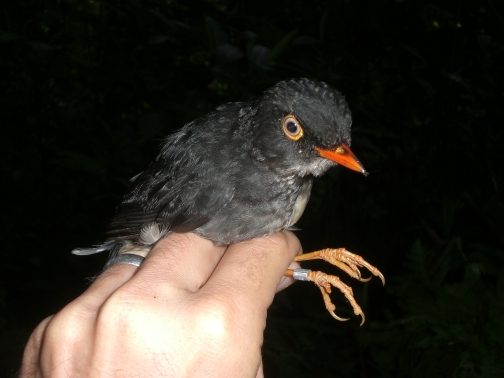
\includegraphics[height=3.5cm,keepaspectratio]{figs/SBNT} %\hfill
    \hspace{0.5cm}
      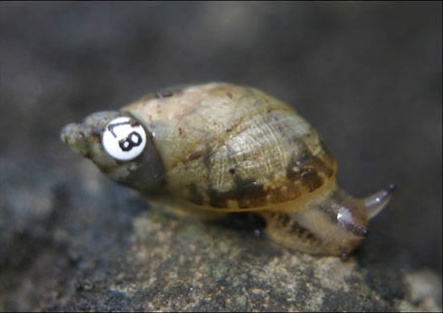
\includegraphics[height=3.5cm,keepaspectratio]{figs/Novisuccinea_chittenangoensis_4}
  \end{center}
\end{frame}




\section{Introduction}


\begin{frame}
  \frametitle{Abundance estimation}
  \large
  Same old equation:
  \[
    \hat{N} = \frac{n}{\hat{p}}
  \]
  \begin{itemize}
    \item $N$ is abundance (population size)
%      \footnote{Density is just $\hat{D} = \hat{N}/A$}
    \item $n$ is the number of individuals detected
    \item $\hat{p}$ is an estimate of detection probability: The probability
      of detecting an individual
  \end{itemize}
  \pause
  \vfill
  \centering
  \Large %\bf
  Most methods differ in how they estimate $p$ \\
\end{frame}




\begin{frame}
  \frametitle{Overview}
  \large
  {%\bf
    Estimating $p$}
  \begin{itemize}[<+->]
    \normalsize
    \item Set traps in a study area and mark each captured individual
    \item Repeat the trapping on $K$ occasions
    \item On each occasion, mark new individuals and record recaptures
    \item If capture probability is high\dots
    \begin{itemize}
      \normalsize
      \item You will detect most of the population on the first
        occasion
      \item Most of the captures on subsequent occasions will be
        recaptures
    \end{itemize}
    \item And vice versa
  \end{itemize}
\end{frame}






\begin{frame}
  \frametitle{Encounter histories}
  {\centering \large $n=5$ individuals captured over 3 sampling occasions \par}
  \vspace{0.3cm}
  \begin{center}
    \small
    \begin{tabular}{lccc}
      \hline
      & Occasion 1 & Occasion 2 & Occasion 3 \\
      \hline
      Animal 1 & 0 & 0 & 1 \\
      Animal 2 & 1 & 1 & 0 \\
      Animal 3 & 1 & 1 & 1 \\
      Animal 4 & 1 & 0 & 0 \\
      Animal 5 & 0 & 1 & 0 \\
      \hline
    \end{tabular}
  \end{center}
  \pause
  \vfill
  \centering
  \large These data tell us about $p$ and hence $N$. Estimation is
  usually acheived using maximum likelihood methods.
\end{frame}








\section{Lincoln-Peterson}


\begin{frame}
  \frametitle{Lincoln-Peterson Method}
  The original method was first used by Pierre-Simon LaPlace to
  estimate the human population in France.   \\
%  \vspace{0.5cm}
  \begin{center}
    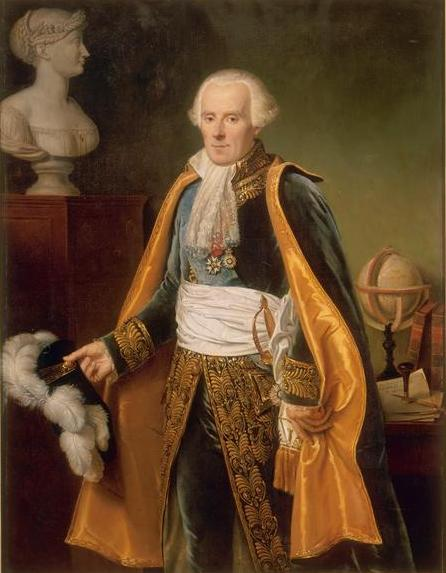
\includegraphics[width=0.4\textwidth]{figs/Laplace} \hspace{0.5cm} \pause
    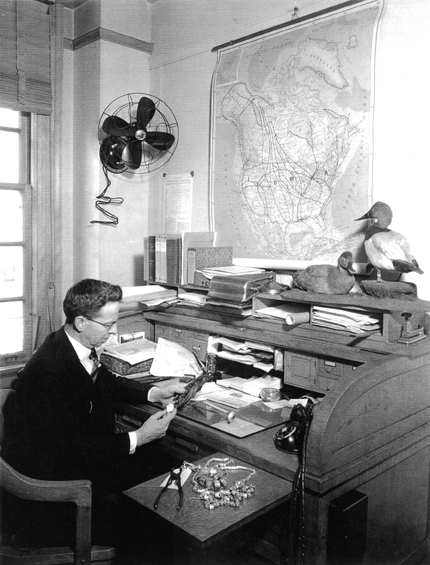
\includegraphics[width=0.4\textwidth]{figs/Frederick_Charles_Lincoln}
  \end{center}
  Later it was used by Lincoln (shown above) and
  Peterson to estimate fish and wildlife populations
\end{frame}


 \begin{frame}
   \frametitle{Lincoln-Peterson Study Design}
   \large %\Large
   \begin{itemize}[<+->]
     \item There are only 2 capture occasions
     \item On the first, $n_1$ animals are captured and marked
     \item On the second, $n_2$ animals are captured and $m_2$ of them
       are recaptures
   \end{itemize}
   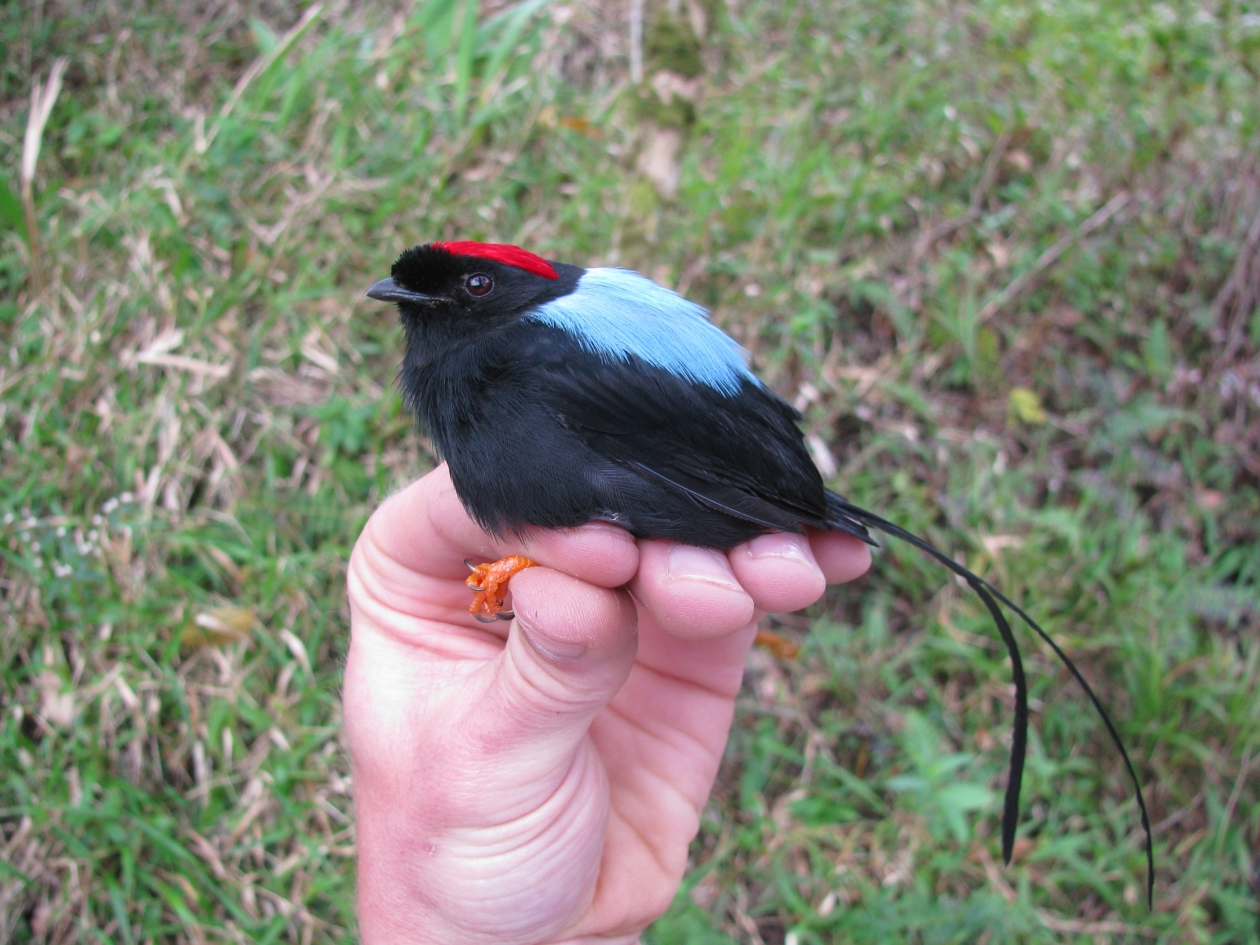
\includegraphics[width=0.45\textwidth]{figs/LTMA} \hfill
   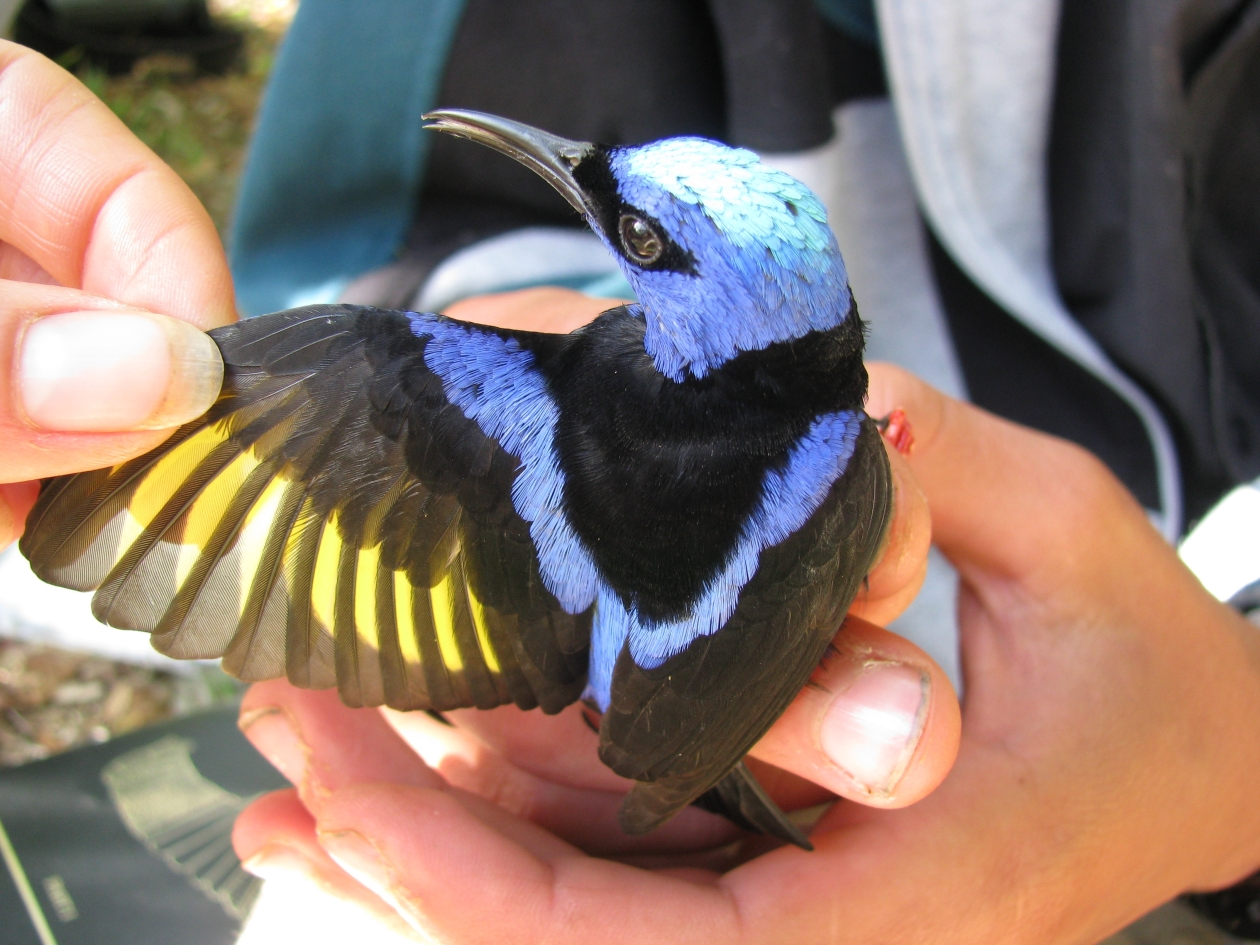
\includegraphics[width=0.45\textwidth]{figs/RLHO}
 \end{frame}



% \begin{frame}
%   \frametitle{Encounter histories}

% \end{frame}









\begin{frame}
  \frametitle{Lincoln-Peterson Abundance Estimator}
  \Large
  How can we use $n_1$, $n_2$, and $m_2$ to estimate $N$? \\
  \vspace{0.3cm}
  \pause
  \LARGE
  \[
    \frac{n_1}{N} = \frac{m_2}{n_2}
  \]
  \pause
  \begin{flushleft}
    {\large And so\dots}
  \end{flushleft}
  \[
    \hat{N} = \frac{n_1n_2}{m_2}
  \]
%  Definitions:
%  \begin{itemize}
%    \item $N$ is population size
%    \item $n_1$ is number of individuals captured on first occasion
%  \end{itemize}
\end{frame}



%\begin{frame}
%  \frametitle{Bias adjustment and variance}
%  Don't worry about it for this course. See the book for teh equations.
%\end{frame}





\begin{frame}
  \frametitle{Lincoln-Peterson Assumptions}
  \large
%  \begin{enumerate}[<+- | visible@+->][\bf \color{PineGreen} (1)]
  \begin{enumerate}[\bf (1)]
    \item<1-> Population closure
      \begin{itemize}
        \large
        \item No births
        \item No deaths
        \item No immigration or emigration
      \end{itemize}
    \item[]
    \item<2-> All individuals are assumed to have the same capture probability
    \item[]
    \item<3-> No tag loss or mis-identification
  \end{enumerate}
%  \vfill
%  \uncover<4->{Because of assumption (1), these methods are referred
%    to as ``closed-population'' mark-recapture}
\end{frame}





\section{$K$-sampler CMR}






\begin{frame}
  \frametitle{$K$-sample CMR}
  \large
  Using more than 2 sampling occasions has many advantages, including
  the ability to account for:
  \begin{itemize}[<+->]
    \large
    \item Temporal variation
    \item Behavioral effects
      \begin{itemize}
        \large
        \item Trap happiness
        \item Trap shyness
      \end{itemize}
    \item Individual heterogeneity
    \item Combinations of the above
  \end{itemize}
\end{frame}


% \begin{frame}
%   \frametitle{Notes}
%   Batch marking
% \end{frame}



\begin{frame}
  \frametitle{Common models}
  \begin{tabular}[h!]{lp{0.8\textwidth}}
    \hline
    Model & Description \\
    \hline
    $M_0$ & The most basic model in which $p$ and $c$ are constant \\
    $M_t$ & $p$ differs among sampling occasions and $p_t=c_t$. \\
    $M_b$ & Behavioral response model in which $p$ and $c$
            differ. Can describe trap happiness or trap shiness. \\
    $M_{tb}$ & A combination of models $M_t$ and $M_b$. \\
    \hline
  \end{tabular}
  \vfill
%  {Parameter definitions \\}
  {where \\}
  \vspace{6pt}
%  \begin{itemize}
%  \item
%  $p$ --- capture probability. The probability of capturing an
%      individual on a single occasion \\
      % \item
%  $p_t$ --- capture probability on occasion $t$ \\
  % \item
%  $c$ --- recapture probability. The probability of capturing an
%      individual that has been captured previously.
%\end{itemize}
  \begin{tabular}[h!]{rl}
%    \hline
%    Parameter & Description \\
%    \hline
    $p =$ & capture probability \\%. The probability of capturing an
      %individual on a single occasion \\
    $p_t =$ & capture probability on occasion $t$ \\
    $c =$ & recapture probability \\%. The probability of capturing an
      %individual that has been captured previously \\
%    \hline
  \end{tabular}

\end{frame}



\section{Removal sampling}


\begin{frame}
  \frametitle{Removal sampling}
  \centering
  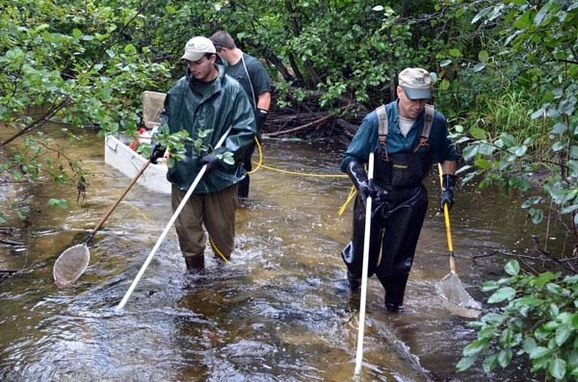
\includegraphics[height=3.2cm]{figs/electrofishing} \hfill
  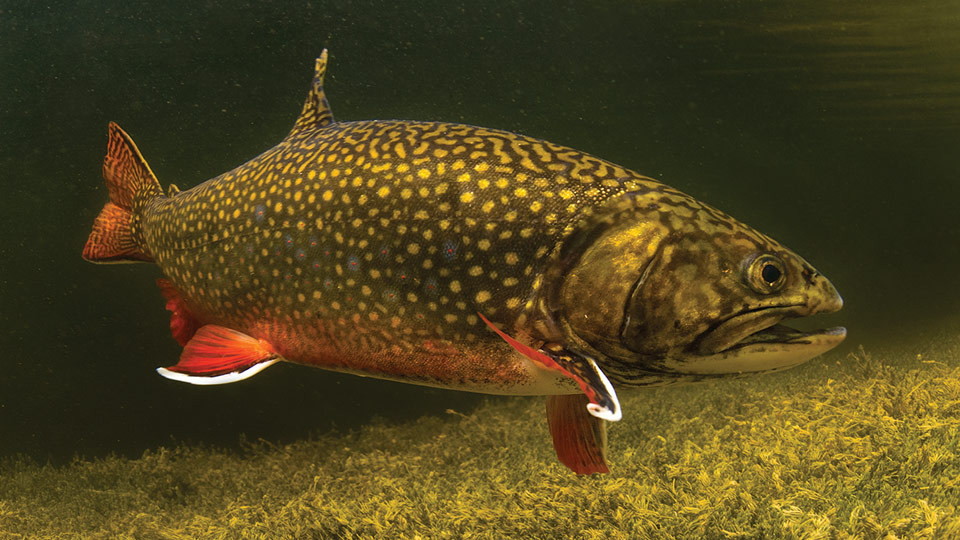
\includegraphics[height=3.2cm]{figs/brook_trout}
  \vfill
  \color{blue}
  \url{https://youtu.be/W3lcHdFyzrQ} \\
\end{frame}


\begin{frame}
  \frametitle{Removal sampling}
  \large
  { Suppose you conduct several electrofishing passes on a single
    stream section, and you remove individuals on each pass. \\}  
  \vfill
  \pause
  { Eventually you should deplete the population. \\}
  \vfill
  \pause
  { The number of captures you would expect on each pass:}
  \begin{center}
    \begin{tabular}{lc}
      \hline
      Pass & Expected captures \\
      \hline
      1 & $pN$ \\
      2 & $p(1-p)N$ \\
      3 & $p(1-p)^2N$ \\
      4 & $p(1-p)^3N$ \\
      \vdots & \vdots \\
      K & $p(1-p)^{K-1}N$ \\
      \hline
    \end{tabular}
  \end{center}
\end{frame}





\begin{frame}[fragile]
  \frametitle{Example}
  % \begin{center}
  \centering
    The rate at which the population is depleted tells us about $p$,
    and therefore how many individuals we missed. \\  
    \vfill
\begin{knitrout}
\definecolor{shadecolor}{rgb}{0.969, 0.969, 0.969}\color{fgcolor}
\includegraphics[width=0.99\linewidth]{figure/rem-1} 
\end{knitrout}
% <<rem2,include=FALSE,echo=FALSE,fig.width=12,fig.height=7>>=
% N <- 100
% p1 <- 0.2
% p2 <- 0.7
% pi1 <- c(p1, p1*(1-p1), p1*(1-p1)^2)
% pi2 <- c(p2, p2*(1-p2), p2*(1-p2)^2)
% pi1[4] <- 1 - sum(pi1)
% pi2[4] <- 1 - sum(pi2)
% set.seed(0324)
% x1 <- drop(rmultinom(1, N, pi1))
% x2 <- drop(rmultinom(1, N, pi2))
% par(mfrow=c(1, 2), mai=c(0.8,0.9,0.8,0.2))
% barplot(x1[1:3], main="", cex.lab=2, cex.main=1.8, cex.axis=1.5,
%         xlab="Occasion", names=1:3, ylab="New captures")
% barplot(x2[1:3], main="", cex.lab=2, cex.main=1.8, cex.axis=1.5,
%         xlab="Occasion", names=1:3, ylab="New captures")
% @
%\includegraphics[width=\textwidth]{lecture13-cap-recapI-rem}
%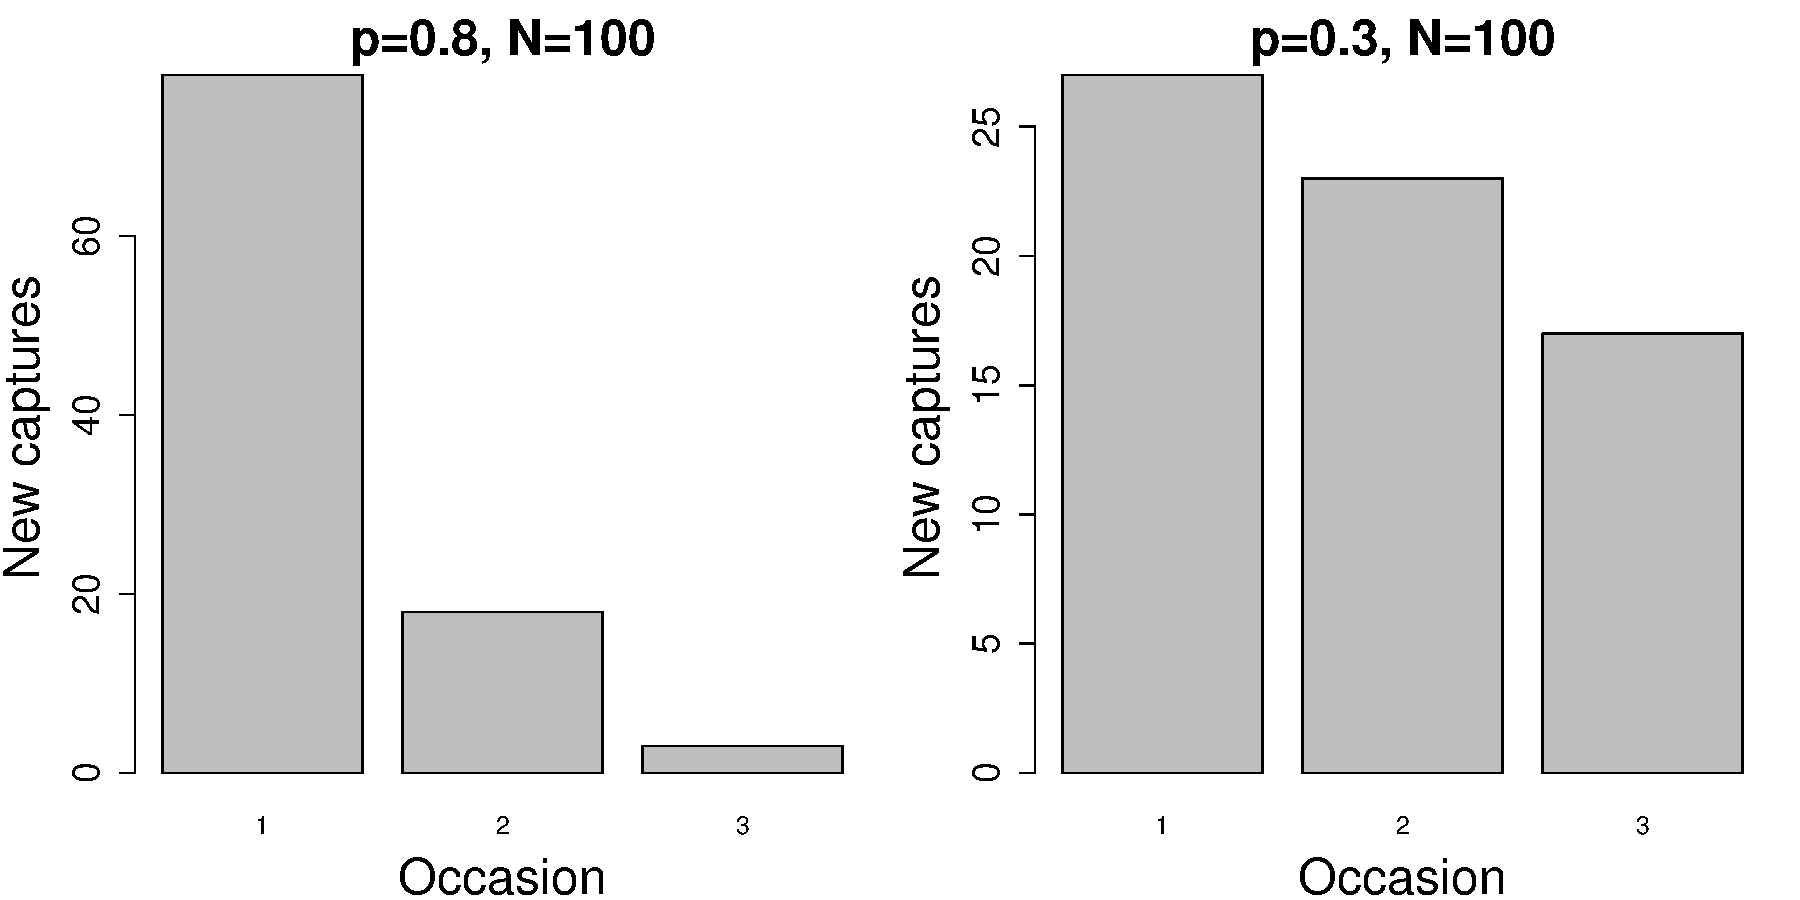
\includegraphics[width=\textwidth]{mark-recap-closedpop-rem}
% \end{center}
\end{frame}








\begin{frame}
  \frametitle{Summary}
  \large
  {\bf Key points}
  \begin{itemize}
    \item Capture-recapture methods use information about recapture
      rates to estimate capture probability and abundance
    \item More advanced methods can be used to estimate density and vital rates
    \item Modern field methods use camera traps or DNA sampling techniques to collect non-invasive capture-recapture data
  \end{itemize}
\end{frame}







\begin{frame}
  \frametitle{Estimating density}
  \large
  {%\bf
    Lingering questions}
  \begin{itemize}
    \item How do we convert abundance to density?
    \item What is the area surveyed?
  \end{itemize}
  \pause
  \begin{center}
    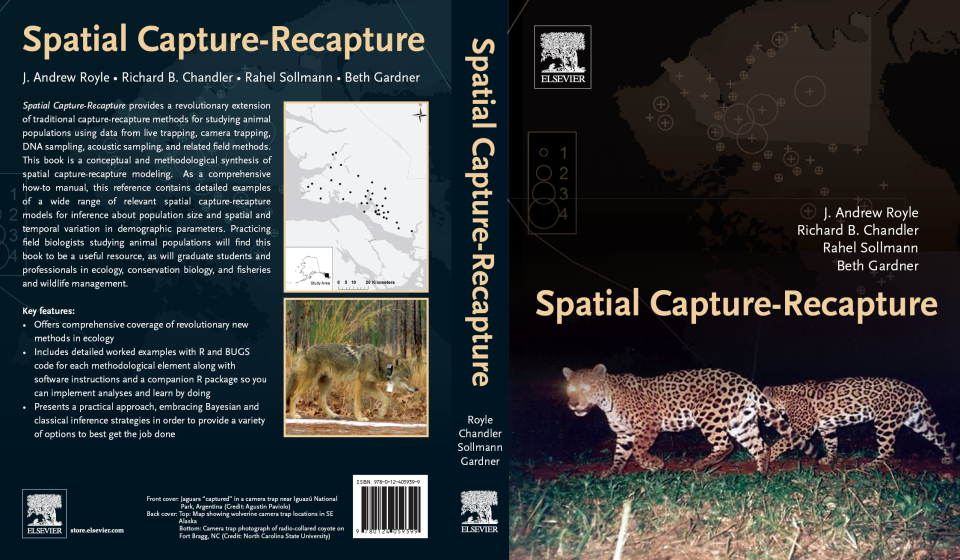
\includegraphics[width=0.75\textwidth]{figs/scrbook}
  \end{center}
\end{frame}




\begin{frame}
  \frametitle{Assignment}
  \centering
  \huge
  Read Chapter 11 \\
\end{frame}



\end{document}


